% ============================================================================
%  Hanoi Urban Noise -- Data Collection Report
%
%  Build:  python3 scripts/10_build_report.py     (writes the inputs, then compiles)
%     or:  latexmk -pdf report.tex                (if the inputs are already there)
%
%  NO NUMBER IS TYPED IN THIS FILE. Everything quantitative arrives through
%  \input{numbers.tex} and the tab_*.tex table bodies, all generated by
%  scripts/10_build_report.py from measurements.csv and models/metrics.json.
%  If a figure here disagrees with models/metrics.json, that is a bug in the
%  generator, not an editorial choice.
% ============================================================================
\documentclass[11pt,a4paper]{article}

\usepackage[T1]{fontenc}
\usepackage[utf8]{inputenc}
\usepackage[english]{babel}
\usepackage{lmodern}
\usepackage{microtype}
\usepackage[margin=25mm,headheight=14pt]{geometry}
\usepackage{array}
\usepackage{booktabs}
\usepackage{graphicx}
\usepackage{xcolor}
\usepackage{amsmath}
\usepackage{fancyhdr}
\usepackage{enumitem}
\usepackage{caption}
\usepackage[hidelinks]{hyperref}

\definecolor{ink}   {HTML}{1A1A1A}
\definecolor{accent}{HTML}{1F5C8B}
\definecolor{warnc} {HTML}{8A4B08}
\definecolor{gray}  {HTML}{6E6E6E}

\hypersetup{colorlinks=true, linkcolor=accent, urlcolor=accent,
            pdftitle={Hanoi Urban Noise -- Data Collection Report},
            pdfauthor={Laurian Jamin, Lucas Zborowski}}

\captionsetup{font=small, labelfont={bf,color=accent}, width=.92\textwidth}
\setlist{itemsep=.25em, topsep=.35em, parsep=0pt}
\renewcommand{\arraystretch}{1.18}

\pagestyle{fancy}\fancyhf{}
\fancyhead[L]{\small\color{gray}Hanoi Urban Noise --- Data Collection Report}
\fancyhead[R]{\small\color{gray}\thepage}
\renewcommand{\headrulewidth}{.4pt}

\newcommand{\LAt}{$L_{A,25\mathrm{s}}$}
\newcommand{\dB}{\ensuremath{\,\mathrm{dB}}}

% A boxed caveat. Used sparingly and always for a limit on what may be concluded.
\newenvironment{caveat}[1]
  {\par\medskip\noindent\begin{minipage}{\linewidth}%
   \color{warnc}\rule{2pt}{\baselineskip}\hspace{.6em}\textbf{#1}\par\vspace{.2em}
   \hspace*{1.4em}\begin{minipage}{\dimexpr\linewidth-1.4em\relax}\small\itshape}
  {\end{minipage}\end{minipage}\par\medskip}

\input{numbers.tex}

% ============================================================================
\begin{document}

\begin{titlepage}
  \centering
  \vspace*{2.5cm}
  {\Huge\bfseries Hanoi Urban Noise Mapping\par}
  \vspace{.6em}
  {\Large\color{gray} Data Collection Report\par}
  \vspace{1.2em}
  {\large \nMeas{} smartphone measurements \quad$\cdot$\quad \nSites{} sites
   \quad$\cdot$\quad \dateMin{} to \dateMax{}\par}
  \vspace{2.2cm}

  \begin{minipage}{.86\textwidth}
    \centering
    \begin{tabular}{@{}ccccc@{}}
      \toprule
      \textbf{Measurements} & \textbf{Sites} & \textbf{\LAt{} range} &
      \textbf{Model $R^2$} & \textbf{$>$ QCVN day} \\
      \midrule
      {\Large\nMeas} & {\Large\nSites} & {\Large\dbMin--\dbMax} &
      {\Large\Rtwohead} & {\Large\excDay\%} \\
      \bottomrule
    \end{tabular}
  \end{minipage}

  \vspace{2.4cm}
  {\large Laurian Jamin \quad$\cdot$\quad Lucas Zborowski\par}
  \vspace{.4em}
  {\small Research interns, ISIMA --- Clermont-Ferrand, France\par}
  \vspace{.3em}
  {\small COSMOS Lab, VinUniversity --- Hanoi, Vietnam\par}
  \vspace{.3em}
  {\footnotesize\color{gray} Supervised by Doanh Nguyen-Ngoc \quad$\cdot$\quad
   With Nguyen Thanh Quang\par}
  \vfill
  {\footnotesize\color{gray}
   Every number in this report is generated from
   \texttt{data/processed/measurements.csv} and \texttt{models/metrics.json}.\\
   None is typed by hand. \quad
   \url{https://github.com/Colauz/noise-modelling-hanoi}\par}
  \vspace{1cm}
\end{titlepage}

\tableofcontents
\clearpage

% ============================================================================
\section{Objective}

Map and characterise urban noise in three contrasting districts of Hanoi, and
predict noise from urban morphology. We follow the Sunbird AI methodology
(\emph{Urban Noise Uganda 61K}, Nsumba et al., 2026): smartphone field collection
plus a morphology-to-noise model, reproduced first on their data and then applied
here.

\begin{caveat}{Measurement status --- read this before any figure below}
  Our target quantity is a 20--30\,s A-weighted level from consumer smartphones,
  denoted \LAt{}. It is \textbf{not} a certified $L_\mathrm{Aeq}$, and not
  $L_\mathrm{den}$ or $L_\mathrm{night}$. The three phones were cross-calibrated
  against \emph{each other}, never against a reference instrument. Contrasts
  between places and between hours are supported; absolute levels are indicative,
  with a plausible bias of \biasLo{} to \biasHi{}\dB{} (section~\ref{sec:refs}).
  No compliance claim is made anywhere in this report.
\end{caveat}

% ============================================================================
\section{Data collection summary}

\begin{table}[h]
  \centering\small
  \input{tab_sites.tex}
  \caption{Field campaign by site. \emph{Roadside} pools the three survey bins
  that mean ``within 10\,m of a road''; the form changed mid-campaign and v1
  offered a single 0--10\,m bin where v2 splits 0--2\,m from 2--10\,m.}
\end{table}

\noindent
\textbf{Zones.} \emph{Ocean Park} --- new high-rise development, with shielding
and active construction. \emph{Vinh Tuy} --- transport infrastructure, heavy
traffic. \emph{Hoan Kiem} --- historic old quarter, narrow streets, pedestrian
zones.

\medskip\noindent
\textbf{Quality control.} Site labels were cross-checked against the GPS fix and
six mislabelled submissions were reassigned to the nearest site centre. No row
was dropped: the raw export holds \nMeas{} submissions and this dataset holds
\nMeas{} rows.

\medskip\noindent
\textbf{Headline findings.} Median \dbMedian\dB{}; \excDay\% of short daytime
samples sit above the QCVN daytime threshold value; levels peak at
\peakHour:00. The delivered model reaches $R^2 = \Rtwohead$
$[\CIheadLo, \CIheadHi]$ under \refLabel{} (section~\ref{sec:model}), against
baselines reported in the same table.

% ============================================================================
\section{Methodology}

\subsection{Field data-collection protocol}

Study zones were mapped in Google Earth and chosen for contrasting typologies
(section~2). At each point we recorded a 20--30\,s reading, with a 10\,s audio
clip, in ODK Collect, submitted live to a KoboToolbox server with an automatic
timestamp and GPS fix. Phones were held at 1.2\,m (SPB positioning) at varied
distances from the road, by three cross-calibrated collectors, from 05:00 to
23:00 with emphasis on rush hours. Weather (Open-Meteo) and spatial context
(OpenStreetMap) are joined afterwards.

\subsection{Reproduction of the Sunbird pipeline}

We reproduced the full Sunbird chain on their Uganda dataset (notebooks 01--06):
cleaning, audio QC, morphology features, figures, surrogate model. Our statistics
match the paper --- median 49\dB{} against their 45--50\dB{}.

\subsection{Model features}

Morphology within 300\,m of each point, from OpenStreetMap: built-area ratio,
road density, intersection count, and distance to the nearest road; plus hour of
day and a weekend flag. The v2 feature set splits distance by road class
(\texttt{dist\_highway}, \texttt{dist\_residential}) and encodes the hour
cyclically.

\subsection{Reference values and measurement status}\label{sec:refs}

\begin{table}[h]
  \centering\small
  \begin{tabular}{@{}lcc@{}}
    \toprule
    \textbf{Reference value} & \textbf{Day (6--21h)} & \textbf{Night (21--6h)} \\
    \midrule
    QCVN 26:2010/BTNMT (Vietnam, ordinary area) & \qcvnDay\dB{} & \qcvnNight\dB{} \\
    \bottomrule
  \end{tabular}
\end{table}

\noindent
The WHO road-traffic guideline values (53 / 45\dB{}) have been \textbf{withdrawn}
from this report. They are $L_\mathrm{den}$ and $L_\mathrm{night}$: annual
averages carrying $+5\dB$ evening and $+10\dB$ night penalties. Comparing them to
a 25\,s daytime sample compares different statistics of different processes. QCVN
is retained because it regulates a level --- but it regulates an $L_\mathrm{Aeq}$
measured with a class 1--2 meter under TCVN 7878-2:2010, a specification our
instrument does not meet either.

\begin{caveat}{Consequence for every exceedance figure in this report}
  It is a \textbf{descriptive statistic of our sample} --- the share of short
  samples above a threshold value --- and never a finding of regulatory
  non-compliance.
\end{caveat}

\noindent
\textbf{Anchoring the absolute bias.} Because we cannot calibrate against a
reference instrument, we bound the bias by comparing our roadside-day stratum to
instrumented campaigns, correcting for the difference expected from the quantity
alone.

\begin{table}[h]
  \centering\footnotesize
  \input{tab_anchors.tex}
  \caption{Anchoring on instrumented literature. The greyed row is grey
  literature --- a secondary source with an undocumented protocol --- and is
  excluded from the interval. Plausible absolute bias of our smartphones:
  \textbf{\biasLo{} to \biasHi\dB{}}. It is reported and \textbf{never applied}:
  the calibration offset is 0.0 for all three collectors.}
\end{table}

\clearpage
% ============================================================================
\section{Data analysis}

\subsection{Temporal patterns}

\begin{figure}[h]
  \centering
  
\includegraphics[width=.94\textwidth]{../figures/analyse_1_horaire.png}
  \caption{Hourly cycle of the median \LAt{} by site. QCVN day and night
  reference values are drawn for orientation only.}
\end{figure}

\begin{figure}[h]
  \centering
  
\includegraphics[width=.82\textwidth]{../figures/analyse_2_jour.png}
  \caption{Day-of-week pattern. Weekend coverage is thinner than weekday
  coverage, and the difference should be read as indicative.}
\end{figure}

\clearpage
\subsection{Sources and exceedances}

\begin{figure}[h]
  \centering
  
\includegraphics[width=.86\textwidth]{../figures/analyse_3_type.png}
  \caption{Level by declared noise category.}
\end{figure}

\begin{table}[h]
  \centering\small
  \input{tab_exceedances.tex}
  \caption{Share of short samples above the QCVN threshold value, by site and
  period. Night rows rest on very few points (\nNight{} measurements fall between
  21:00 and 06:00 in the whole campaign) and are reported for completeness, not
  for inference.}
\end{table}

\begin{figure}[h]
  \centering
  
\includegraphics[width=.86\textwidth]{../figures/analyse_4_depassement.png}
  \caption{Share of short samples above the QCVN daytime threshold value, by
  hour. A bias of a few decibels moves this curve substantially, which is why the
  interval of section~\ref{sec:refs} is quoted with it.}
\end{figure}

\clearpage
\subsection{Traffic and weather}

\begin{figure}[h]
  \centering
  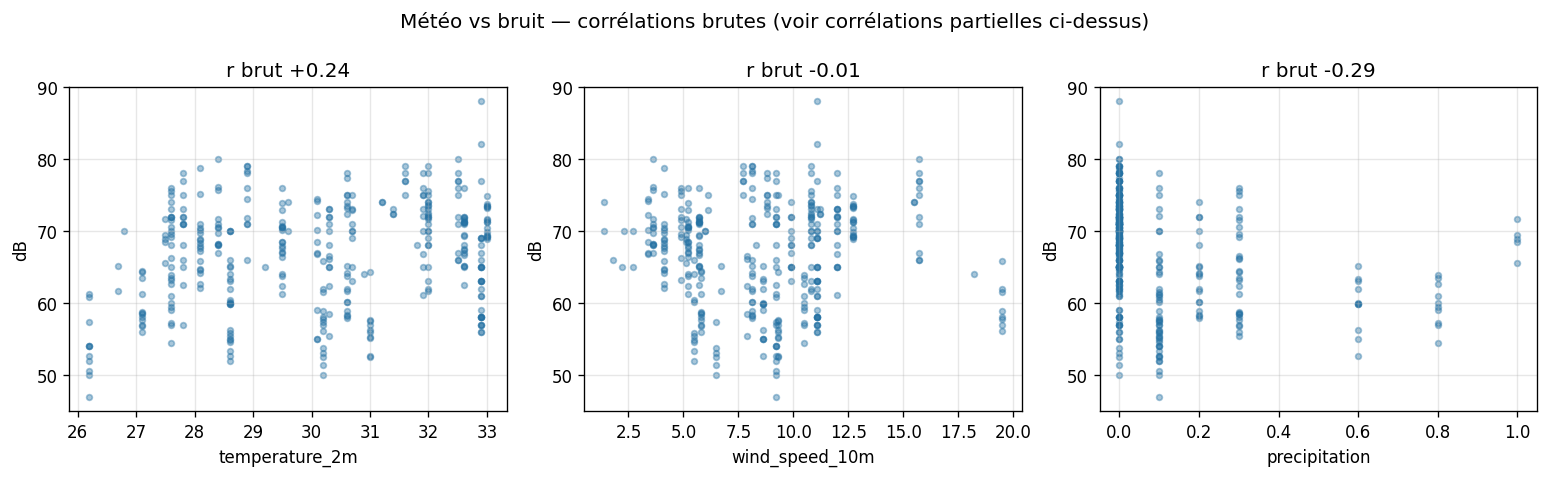
\includegraphics[width=.86\textwidth]{../figures/analyse_5_meteo.png}
  \caption{Weather covariates against level. Temperature, wind and precipitation
  are joined from Open-Meteo at the hour of measurement.}
\end{figure}

\noindent
\textbf{Traffic videos.} 147 timestamped videos were counted with YOLOv8 and
ByteTrack, producing flow by class from line crossings rather than density.
Non-negative energy regression against the matched levels returns \textbf{zero
coefficients} for motorcycles and cars. Two causes are identifiable and neither
is acoustic: speed is unobservable without a ground homography, and the field of
view is not georeferenced, so the source--receiver distance is discarded.

\begin{caveat}{The detector has never been validated against manual counts}
  Precision, recall and MAPE per class are unknown, and two-wheeler
  under-detection is expected but unquantified. \textbf{Modal shares must not be
  published until it is done.} One day of manual counting on ten videos turns an
  open-ended limitation into a quantified uncertainty; it is the highest
  value-per-effort task left in the project.
\end{caveat}

\clearpage
% ============================================================================
\section{Predictive model}\label{sec:model}

\subsection{How performance is measured}

An earlier version of this report quoted $R^2 = 0.45$ from a cross-validation
grouped on cells of about 110\,m. The morphology features aggregate over a disc
of \textbf{radius \bufferM\,m}: two points 110\,m apart share more than 85\,\% of
that disc, so the model saw near-twins of its test points during training. That
score was not out-of-sample and \textbf{has been withdrawn} (Roberts et al.\
2017, \emph{Ecography}).

Every model below is scored under three splits, on exactly the same folds:

\begin{enumerate}
  \item \textbf{Block-CV \blockM\,m} --- square blocks in UTM 48N,
        \texttt{GroupKFold} on the block identifier. \nBlocks{} blocks. The
        permissive protocol.
  \item \textbf{Buffered leave-one-out \bufferM\,m} --- for each point, train on
        all points more than \bufferM\,m away from it. \textbf{The reference
        protocol}: it matches the feature radius and has no split randomness.
  \item \textbf{Leave-one-site-out} --- generalisation to an unseen urban
        typology.
\end{enumerate}

\noindent
Every score carries a 95\,\% interval bootstrapped \textbf{by block} over
\nBootstrap{} resamples, not by point: resampling correlated points would give an
interval far too narrow.

\subsection{Model comparison}

\begin{table}[h]
  \centering\small
  \input{tab_models.tex}
  \caption{All models on identical splits. The delivered model is in bold and is
  selected \textbf{by code} under the reference protocol; the choice is written
  into \texttt{models/metrics.json} and read by the export, so nothing downstream
  can silently substitute another.}
\end{table}

\noindent
\textbf{The ranking inverts between the permissive split and the strict ones.}
The hybrid architecture --- a physical core corrected by a LightGBM fitted to the
residual, the design this team had itself recommended --- leads under block-CV
($\BcvHybrid$ against $\BcvPhysical$ for the bare core) and loses under both
strict protocols ($\RtwoHybrid$ against $\Rtwohead$ under \refLabel{}). It is
therefore reported as \textbf{tested and rejected at this sample size}, not
deferred to future work. The residual is trained at every run and
\texttt{apply\_residual} is \applyResid{}.

\subsection{The delivered model}

A line-source attenuation kernel with three positive parameters and no
morphological input at all:
\[
  E \;=\; \frac{A_\mathrm{hw}}{\max(d_\mathrm{hw}, D_0)}
        + \frac{A_\mathrm{res}}{\max(d_\mathrm{res}, D_0)} + B,
  \qquad L = 10\log_{10} E,
\]
with $A_\mathrm{hw} = \Ahw$, $A_\mathrm{res} = \Ares$ and $D_0 = \Dzero$\,m.

\begin{caveat}{The background term is not identifiable from these data}
  $B$ is fitted to $\Bbg\dB$, a boundary solution. Called a three-parameter
  model, it behaves as a two-parameter one: \nMeas{} points over \nSites{} sites
  do not constrain a floor.
\end{caveat}

\noindent
Under the reference protocol: $R^2 = \Rtwohead$ $[\CIheadLo, \CIheadHi]$,
$\mathrm{MAE} = \MAEhead\dB$, $\mathrm{RMSE} = \RMSEhead\dB$, against a data
spread of $\dbSd\dB$. \textbf{A typical prediction is wrong by about
\MAEhead\dB{}} --- a factor of three in acoustic energy. That is enough to
support a contrast and nowhere near enough to support an assessment.

\medskip\noindent
Note also that the confidence interval of the delivered model overlaps that of
the plain $\log(d_\mathrm{road})$ regression ($R^2 = \RtwoDistRoad$). The
ordering between those two is not statistically separated at this sample size,
and should not be reported as though it were.

\subsection{Generalisation to an unseen typology}

Under leave-one-site-out, the learned models collapse towards or below zero while
the physical kernel retains most of its score. With three sampled typologies the
number of independent morphological configurations available is close to three,
whatever the number of points --- so maps are clipped to the sampled envelope
regardless of the score.

\clearpage
% ============================================================================
\section{Agent-based simulation}

The GAMA model (\texttt{simulation/gama/hanoi\_noise.gaml}) reads the exported
40\,m grid and adds receiver agents, mobile vehicles for visualisation, and
construction sites calibrated in energy. Tier~1 exposes sliders for hour, traffic
volume and mitigation.

\medskip\noindent
\textbf{One correction worth recording.} The traffic multiplier scales the
\emph{traffic share} of the energy and never the background. Applied to total
energy, it double-counts the background and inflates the apparent benefit of
mitigation: the claimed gain from pedestrianisation fell from $7.0\dB$ to
$3.5\dB$ once the multiplier was applied correctly.

\medskip\noindent
Measured flow is injected only within 150\,m of a measurement point. The exported
zone extends 400\,m beyond the survey envelope, and spreading flow uniformly over
every street in it left the Hoan Kiem lake loop empty although every video had
been filmed there.

\begin{figure}[h]
  \centering
  
\includegraphics[width=.9\textwidth]{../figures/validation_simulation.png}
  \caption{Simulated against measured levels. The simulation reproduces the
  spatial and temporal ordering; it does not reproduce the spread, which is
  expected given that features aggregated over \bufferM\,m cannot resolve the
  facade/courtyard contrast.}
\end{figure}

\clearpage
% ============================================================================
\section{Limitations, stated plainly}

\begin{itemize}
  \item \textbf{The learned component does not survive an honest spatial split.}
        The hybrid architecture leads under the permissive \blockM\,m block split
        and loses under both strict ones. The delivered model is the bare
        physical core; the residual is trained but not applied. Morphology
        aggregated over \bufferM\,m adds no measurable value over the two
        distance terms alone.

  \item \textbf{Absolute calibration.} The three phones are calibrated against
        each other, never against a reference instrument. A bias common to all
        three (\biasLo{} to \biasHi\dB{}, bounded by anchoring on instrumented
        Vietnamese campaigns) is invisible in our data by construction. The field
        campaign is closed and this cannot be repaired retrospectively.

  \item \textbf{Measurement quantity.} A 20--30\,s sample is not the
        $L_\mathrm{Aeq}$ of any regulatory reference period. A single horn burst
        moves it by several decibels --- horn events reach $+17\dB$ in Vietnamese
        traffic. This variance is a property of the quantity and caps the $R^2$
        any spatial model can reach.

  \item \textbf{Generalisation.} Three sampled typologies bound every
        generalisation claim. The physical model extrapolates markedly better
        than the learned ones, but three typologies remain three.

  \item \textbf{Spatial resolution.} Features are aggregated over a \bufferM\,m
        radius, so adjacent 40\,m cells share more than 98\,\% of their disc. The
        map cannot resolve the facade/courtyard contrast, which reaches
        10--15\dB{} in dense fabric: predicted levels are visibly flatter than
        measured ones.

  \item \textbf{Temporal coverage.} Only \nNight{} measurements fall between
        21:00 and 06:00, and none between 00:00 and 05:00 --- although that is
        the period with the strictest threshold. One season only.

  \item \textbf{Traffic videos.} Counts are real flow, from tracking and line
        crossing, but speed remains unobservable without a ground homography and
        the field of view is not georeferenced, so distance is discarded. The
        detector was never validated against manual counts.
\end{itemize}

% ============================================================================
\section{Next steps}

\begin{itemize}
  \item \textbf{Richer physics, not more learning.} The three-parameter
        line-source core already beats every learned variant. The next gain
        should come from a real propagation model --- CNOSSOS-EU via
        NoiseModelling: screening, reflections, canyon geometry --- not from more
        capacity fitted to \nMeas{} points. A learned residual should be
        re-tested only once the sample covers more typologies; on this one it
        degrades generalisation.

  \item \textbf{Anchor the absolute scale.} A class 1--2 sound level meter, or a
        94\dB{} / 1\,kHz acoustic calibrator, turns the bias interval into a
        measured correction. Everything downstream inherits it.

  \item \textbf{Traffic.} Flow by class is measured; \emph{speed} is the missing
        half. Estimate it from track displacement under a ground homography,
        which also georeferences the field of view and so restores the
        source--receiver distance. Validate the detector against manual counts
        first.

  \item \textbf{More typologies.} A fourth and fifth contrasting urban fabric
        would do more for the generalisation claim than any modelling change.

  \item \textbf{Data publication.} Deposit measurements, forms and code with a
        DOI, and add an ethics statement covering the public-space video
        recordings.
\end{itemize}

% ============================================================================
\section{Summary}

\nMeas{} smartphone measurements across \nSites{} districts document a consistent
exposure pattern in space and time. The delivered model is a three-parameter
physical line-source law: $R^2 = \Rtwohead$ $[\CIheadLo, \CIheadHi]$,
$\mathrm{MAE} = \MAEhead\dB$ under \refLabel{} --- ahead of a $\log(\text{distance})$
regression ($\RtwoDistRoad$), a six-feature LightGBM ($\RtwoLgbmFull$) and the
physics-plus-ML hybrid built to improve on it ($\RtwoHybrid$).

\medskip\noindent
Three negative results are the contribution. Every learned elaboration gains
under a permissive spatial split and loses under a strict one. Cross-city
transfer from Uganda fails. Video counts yield no emission coefficient, as
density or as flow. \textbf{We claim contrasts, not absolutes.}

\vfill
\noindent\rule{\linewidth}{.4pt}\par
{\footnotesize\color{gray}
Generated by \texttt{scripts/10\_build\_report.py} from
\texttt{data/processed/measurements.csv} and \texttt{models/metrics.json}.
Delivered model: \texttt{\deliveredKey} --- \deliveredName{}, selected under
\refLabel{}. Reproduce with \texttt{make report}.\par}

\end{document}
